% !TEX root = template.tex

\section{Introduction}

Here goes the introduction. We also cite the nice book by \citet{Pinedo:2012}.
This might be a book with interesting topics, but concurrent time-stamping has also been addressed before~\cite{Dolev97}.
In this work, \citet{Dolev97} presented the first bounded implementation of a concurrent time-stamp system.


\section{Algorithm X}

Table~\ref{tab:related_algorithms} shows a summary of related algorithms.

\begin{table}[h]
\centering
\captionabove{Related algorithms and their complexity.}
\label{tab:related_algorithms}
\begin{tabular}{ll}
\toprule 
algorithm & complexity \\
\midrule
algorithm Y & $\mathcal{O}(n)$ \\
algorithm Z & $\mathcal{O}(n \log{n} )$ \\
\bottomrule
\end{tabular}
\end{table}

\section{Evaluation of Algorithm X}


\subsection{Evaluating the Running Time of Algorithm X}

The run-time of our algorithm is shown in Figure~\ref{fig:runtime}.
We can observe that the run-time of our algorithm increases linearly with the message size.
Since we target a system with a run-time of less than \SI{10}{\second}, the maximum message size should be \SI{128}{\byte}.

\begin{figure}[h]
\centering
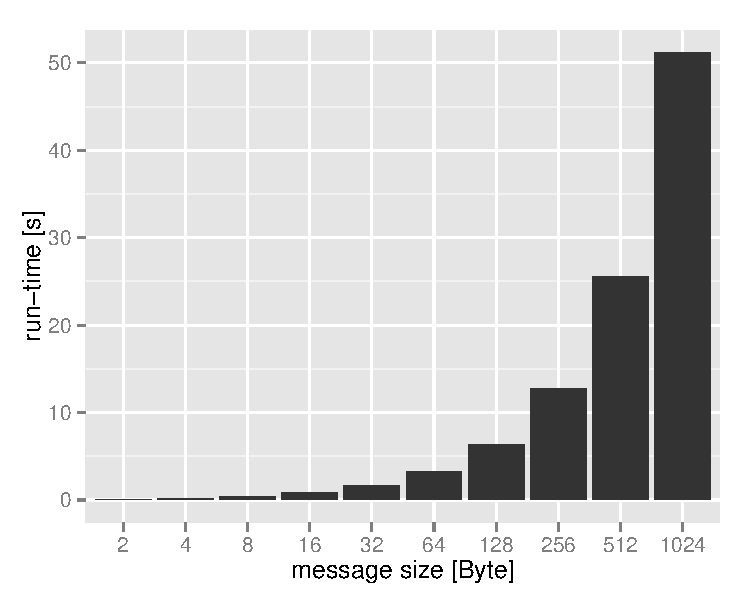
\includegraphics[width=.5\linewidth]{figures/runtime}
\caption{Run-time of algorithm X on machine Y.}
\label{fig:runtime}
\end{figure}

\subsection{Evaluating the Space Requirements of Algorithm X}

Now, we investigate the space requirements of the algorithms listed in Table~\ref{tab:related_algorithms}.


\section{Summary}
We summary the contribution of the papers and this seminar paper.
